\documentclass{article}
\usepackage{amsmath}  % 数学符号包
\usepackage{amssymb}  % 更多数学符号
\usepackage{enumitem} % 列表样式
\usepackage{fancyhdr} % 页眉设置
\usepackage{geometry} % 页面设置
% \usepackage[UTF8]{ctex}
\usepackage{bm}
\usepackage{amsthm}
\usepackage{tikz}
\everymath{\displaystyle}  % 让所有数学模式都使用 \displaystyle
\newcommand{\lb}{\left\llbracket}
\newcommand{\rb}{\right\rrbracket}


\geometry{a4paper, margin=1in}


\pagestyle{fancy}
\fancyhf{}
\fancyhead[C]{Discrete Math Homework 16}
\fancyhead[R]{2024.12.22}


\title{Discrete Math Homework 16}
\author{noflowerzzk}
\date{2024.12.22}


\begin{document}
\maketitle

\section{}

a), b), d), f)

\section{}

\begin{proof} \quad
    \begin{itemize}
        \item If the simple path passes through $w$, due to the path is simple, it's obvious that $d(u, v) = d(u, w) + d(w, v)$.
        \item If $d(u, v) = d(u, w) + d(w, v)$, let the path from $u$ to $w$ is $u = x_0, x_1, \cdots, x_n = w$, $d(u, v) = n$, let the path from $v$ to $w$ is $v = y_0, y_1, \cdots, y_m = w$, $d(v, w) = m$, then connect the two path $u = x_0, x_1, \cdots, x_n = w = y_m, y_{m - 1}, \cdots, y_0 = v$, then length of the path is $m + n = d(u, v)$, so the path is the simple path between $u, v$, i.e. is passes through $w$.
    \end{itemize}
\end{proof}

\section{}

Let the root denoted by $r$.

\begin{itemize}
    \item [(a)] \begin{proof}
        For any $(u, v) \in R_1$, there is a unique simple path from $r$ to $v$ which passes through $u$ and $u \neq v$, i.e. $u$'s level is strictly lower than $v$, so $(u, v) \in R_2$. So $R_1 \subseteq R_2$.
    \end{proof}
    \item [(b)] \begin{proof}\quad\\ \quad \\
        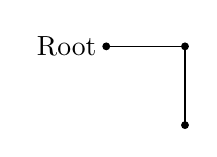
\begin{tikzpicture}
            \fill(0, 0) circle(.05);
            \node at (0, 0) [left] {Root};
            % \node at (Root)[]{Root}; 
            \fill (1, 0) circle(.05);
            \fill (1, -1) circle(.05);
            \draw (0, 0) -- (1, 0);
            \draw (1, 0) -- (1, -1);
        \end{tikzpicture}
    \end{proof}
    \item [(c)] \begin{proof} \quad \\ \quad \\
        \begin{tikzpicture}
            \fill(0, 0) circle(.05);
            \node at (1, 0) [right] {Root};
            % \node at (Root)[]{Root}; 
            \fill (1, 0) circle(.05);
            \fill (1, -1) circle(.05);
            \fill (1, -2) circle(.05);
            \draw (0, 0) -- (1, 0);
            \draw (1, 0) -- (1, -1);
            \draw (1, -1) -- (1, -2);
        \end{tikzpicture}
    \end{proof}
\end{itemize}

\section{}

\begin{proof}
    According to the definition of ancestor, there is a unique path from root $r$ to $w$ which passes through $u, v$, i.e. $r = x_0, x_1, \cdots, x_n = w$, $\exists i, j \in \{1, 2, \cdots, n\}$, $u = x_i, v = x_j$.\\
    If $i = j$, then $u = v$.\\
    If $i < j$, then $r = x_0, x_1, \cdots, x_i = u, \cdots, x_j = v$, so $u$ is the ancestor of $v$. \\
    If $i > j$, then similarly $v$ is the ancestor of $u$.
\end{proof}

\section{}

Let $P(G)$ denote that the rooted tree $G$ is a tree such that every internal vertex has at least two children, $Q(G)$ denote that $G$'s leaves is more than its internal vertexes, i.e. $n(\text{internal vertexes}) \leqslant n(\text{leaves}) - 1$. \\

\begin{proof}\quad
    \begin{itemize}
        \item Let $T_1$ is a root tree with height of 1, then the number of internal vertex is 1 and the number of leaves is more than 2. So $Q(T_1)$.
        \item Assume that all the root tree $T_k$ with $P(T_k)$ and height less than $n$ satifies $Q(T_k)$, then for any rooted tree $T$ with height $n$ and $P(T)$, let $T$'s root be $r$, then it has $t\ (t \geqslant 2)$ children.\\
        All the subtree with root of $r$'s children $(S_1, S_2, \cdots, S_p)$ satifies property $P$ and their height less than $n$, so according to the assumption, their leaves are more than their internal vertexes. so
        \begin{align*}
            n(\text{internal vertexes of T}) &= 1 + \sum_{i = 1}^{p}n(\text{internal vertices of }S_i) & \quad (p \geq 2)\\
            &\leqslant 1 - p + \sum_{i = 1}^{p}n(\text{leaves of }S_i) \\
            &< n(\text{leaves of }T)
        \end{align*}
    \end{itemize}
    According to inducing principle, all the rooted trees such that every internal vertex has at least two children have more leaves than internal vertexes.
\end{proof}

\end{document}